%************VERSUCHSDURCHFÜHRUNG & MESSERGEBNISSE***********
\section{Execution}
\label{sec:execution}

This sections serves as documentation on how the results as described in Section \ref{sec:summary} might be reproduced. Instructions are based on the assumption that an environment with suitable equipment such as described in Sections \ref{sec:setup} and \ref{sec:equipment} is used and set up accordingly.

\subsection{Laser Source and Safety}
\label{sec:laser-source-and-safety}

All experimental steps described in subsequent sections require the infrared laser source to be operational, for which the main switch needs to be activated. Additionally, there is a cover at the output of the laser source blocking the outgoing beam that needs to be opened during measurement.

For safety reasons, this cover is to remain closed while changes to the setup are made. Furthermore, safety goggles need to be used and reflective apparel such as watches or rings need to be removed. The eyes of the experimentators must strictly remain well above the path of the laser beams.

\subsection{Beam Positioning}
\label{sec:execution:beam-positioning}

For the laser beam to be measured by the grating spectrometer, it needs to be directed from the output of the laser source towards the input aperture of the spectrometer. This is achieved by directing it via a series of dielectric mirrors, which are positioned and aligned such that on one hand the SHG stage and the iodine cell can be traversed by the beam, while on the other hand the beam reaches the aperture of the spectrometer in a correct angle.

For a wavelength of \SI{1030}{\nm}, the mirrors of type E03 are used, while for beams after the SHG stage with a desired wavelength of \SI{515}{\nm} the type E02 mirrors are utilised. Using the latter for beams in the visible green spectrum ensures that a portion of remaining infrared photons are not reflected, effectively filtering them on the way to the spectrometer.

As described in Section \ref{sec:setup}, the bases for the optical elements used in this experiment can be positioned and fixed on a grid of tapped holes. While the bases allow for vertical adjustment as well as crude rotation with respect to the vertical axis, the mounts allow for fine-tuned vertical and horizontal tilting of the mirrors, thus enabling alignment of the laser beam as desired.

One strategy that proves to be advantageous is to locate the mirrors in such a way that the beam follows a path containing only angles of approximately \SI{90}{\degree}, for which the reflection angle relative to each mirror is approximately \SI{45}{\degree}. For this approach the grid of tapped holes in the table can be used as a rough reference, while additionally the sensitivity for changes in mirror angle are minimized.

As shown in Figure \ref{fig:execution:aperture}, the grating spectrometer exhibits a dedicated adjustable mirror for directing the laser beam towards the aperture. There are covers at both the mirror and the aperture, each containing a special hole to be used for properly adjusting the laser beam while the covers are closed. When correctly adjusted, the laser beam hits both the hole at the mirror as well as the hole at the cover of the aperture. During measurement, the cover at the mirror is always to be opened.

\begin{figure}[H]
    \centering
    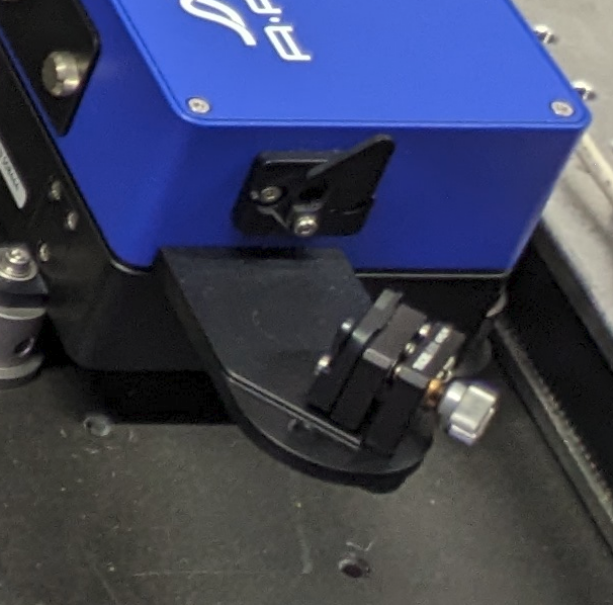
\includegraphics[width=0.45\textwidth]{graphics/aperture.png}
    \caption{Aperture and dedicated mirror at the grating spectrometer.}
    \label{fig:execution:aperture}
\end{figure}

The overall procedure for directing the beam towards the spectrometer as desired involves stepwise adjustment of the mirrors starting from the laser source and going towards the spectrometer, followed by iterative fine-tuning of each mirror both in height and rotation.

\subsection{Measurement Procedure}
\label{sec:execution:measurement-procedure}

In order to measure the power of the beam, the power meter as documented in Table \ref{tab:equipment} and depicted in Figure \ref{fig:execution:powermeter} is used. The photodiode sensor needs to be connected to the console via cable and placed such that it is hit by the laser beam. For all measurements described in the subsequent sections, the relative measurement mode is activated by pressing the "$\Delta$" button. While the range is always set to automatic mode, the wavelength is set manually to either $\SI{1030}{\nm}$ for the infrared laser or $\SI{515}{\nm}$ for the frequency-doubled laser, which can be achieved by navigating the menu using the arrow and "OK" buttons. It should be noted here that setting the wavelength is merely used for calculating the power - the power meter does not filter unrelated wavelengths.

\begin{figure}[H]
    \centering
    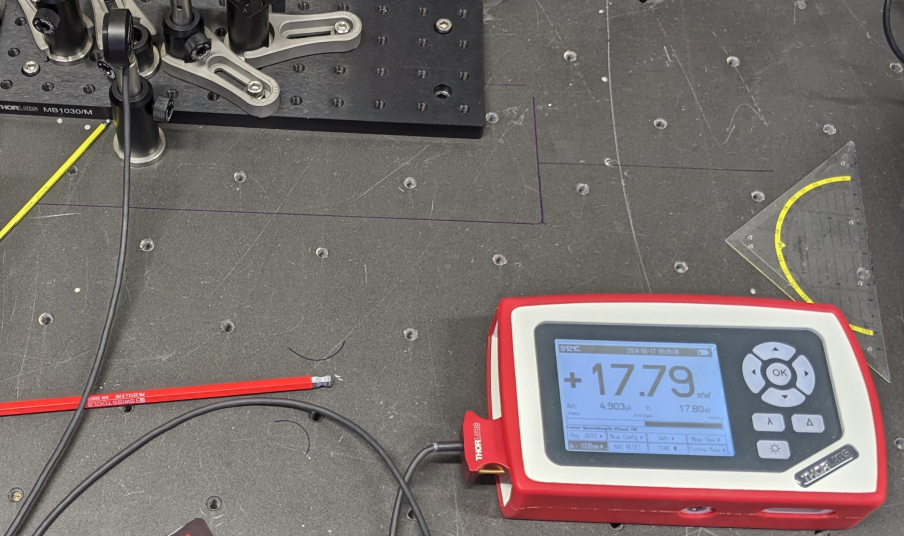
\includegraphics[width=0.45\textwidth]{graphics/power-meter.png}
    \caption{Power meter consisting of console and sensor.}
    \label{fig:execution:powermeter}
\end{figure}

For the grating spectrometer, which needs to be set up as described in Section \ref{sec:execution:beam-positioning}, measurement needs to be started by clicking the "Start" button in the bottom right corner. The view of the measured spectrum is updated in realtime and can be zoomed in by clicking the magnifying glass button or reset via the crosshair button, which are both located in the bottom right corner of the user interface.

The "View" and "Setup" menus in the top left corner of the interface allow to enable averaging of the measured spectra for up to $256$ measurements, which proves beneficial for reducing noise. The menus also allow to confine the wavelength of the spectra to a specific domain, increasing the available resolution when considering specific regions of interest.

For exporting measured spectra, the "File$~$\textrightarrow$~$Spectrum to file" operations are used. It is important to notice that the used version of the software as documented in Table \ref{tab:equipment} updates the data until the instant where the "Save" button in the file dialog is being hit. Using "File$~$\textrightarrow$~$Spectrum as reference" an existing spectrum may be loaded, which in addition to the spectrum currently measured will be displayed in the user interface. This allows to visually compare current measurements with previously recorded spectra for reference.

\begin{figure}[H]
    \centering
    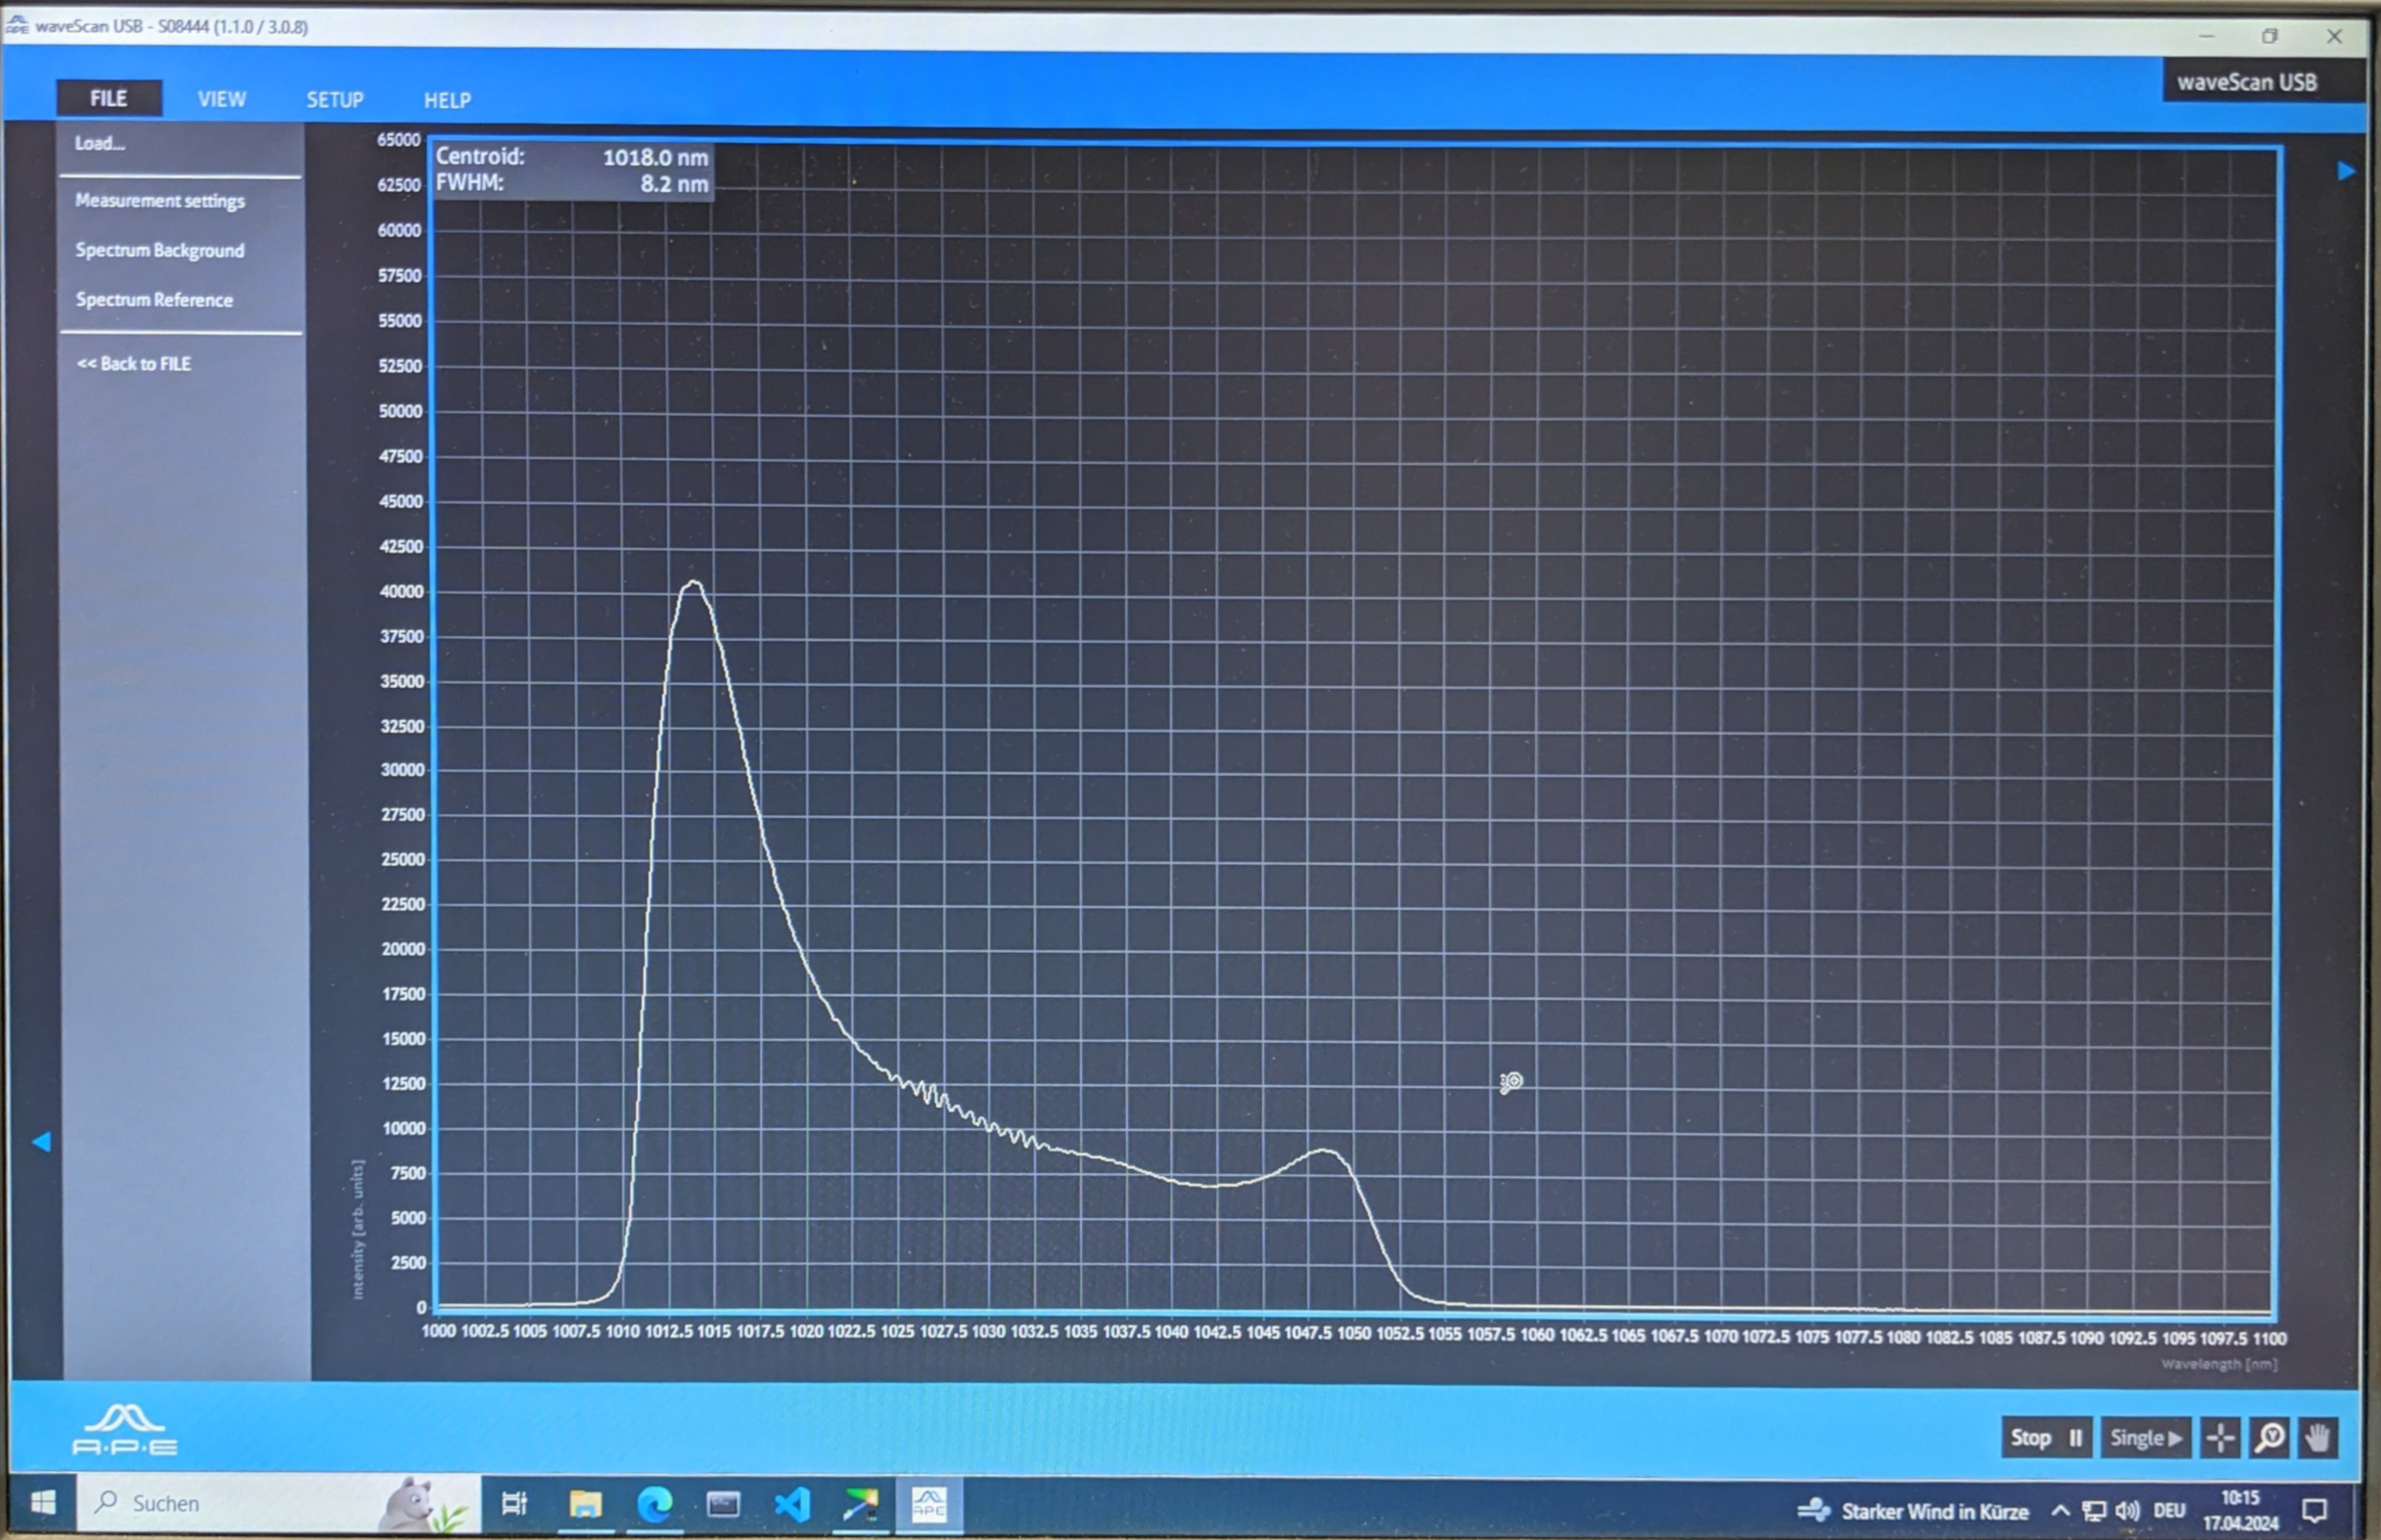
\includegraphics[width=0.45\textwidth]{graphics/wave-scan.jpg}
    \caption{Graphical interface of APE waveScan.}
    \label{fig:execution:wave-scan}
\end{figure}

\subsection{Laser Source Characterization}
\label{sec:execution:infrared-characterization}

In a first step, the infrared laser beam emitted by the laser source is characterized. As depicted in Figure \ref{fig:setup:power}, operating as described in sections \ref{sec:execution:beam-positioning} to \ref{sec:execution:measurement-procedure}, the average power output is measured for a wavelength of \SI{1030}{\nm} using the power meter. Taking into account the uncertainty of the photodiode sensor as documented in Table \ref{tab:equipment}, which is specified as $\pm \SI{7}{\percent}$ in the used range, and further considering deviations of the laser source from the wavelength of \SI{1030}{\nm} used by the console for calculating the power, a combined uncertainty of $\pm \SI{10}{\percent}$ is assumed. The average power of the infrared source therefore reads $P_{IR} = \SI{17.8(18)}{\mW}$.

In order to be able to obtain the central wavelength as well as FWHM of the infrared laser, the spectrometer is used to measure and export the spectrum in a format such as shown in Table \ref{tab:execution:infrared-characterization}. For this, the procedure as described in sections \ref{sec:execution:beam-positioning} to \ref{sec:execution:measurement-procedure} is followed. The setup for obtaining the spectrum is shown in Figure \ref{fig:setup:basic}.

\begin{table}[H]
    \centering
    \caption{Intensity spectrum for the infrared laser. \\
    $\lambda$ = Wavelength, $I$ = Intensity count}
    \label{tab:execution:infrared-characterization}
    \begin{tabular}{ccccc}
    \hline
    $\lambda$ / nm & $I$ / 1 \\ \hline
    1000  & 28  \\
    \vdots & \vdots  \\
    1100 & 216 \\ \hline
    \end{tabular}
\end{table}

\subsection{SHG Characterization}
\label{sec:execution:shg-characterization}

In a second step, the SHG stage, which is described in more detail in Section \ref{sec:setup}, is added to the setup as shown in Figure \ref{fig:setup:shg}. This involves proper re-alignment of the beam path using type E02 mirrors, which is described in Section \ref{sec:execution:beam-positioning}, as well as adjustment of all optical elements of the SHG. 

Rotating the non-linear crystal such that phase matching required for successful SHG is achieved and based on this the amount of frequency-doubled photons is maximized is of particular importance. Rotation of the crystal is conveniently afforded by the corresponding mount.

Analogous to the procedure in Section \ref{sec:execution:infrared-characterization}, the power meter is used to obtain the average power of the green laser beam. After configuring the wavelength of \SI{515}{\nm} at the console, for which the photodiode sensor specifies an uncertainty of $\pm \SI{3}{\percent}$, and further considering significant deviations of the SHG output from the wavelength of \SI{515}{\nm} (including remaining infrared photons) used by the console for calculating the power, a combined uncertainty of $\pm \SI{15}{\percent}$ is assumed. The average power of the SHG source therefore reads $P_{SHG} = \SI{3.7(6)}{\mW}$.

The spectrometer is used to obtain and export the spectrum just as described in Section \ref{sec:execution:infrared-characterization}. The resulting data is shown in Table \ref{tab:execution:shg-characterization}.

\begin{table}[H]
    \centering
    \caption{Intensity spectrum for the SHG output. \\
    $\lambda$ = Wavelength, $I$ = Intensity count}
    \label{tab:execution:shg-characterization}
    \begin{tabular}{ccccc}
    \hline
    $\lambda$ / nm & $I$ / 1 \\ \hline
    500  & 10.6  \\
    \vdots & \vdots  \\
    530 & 16.6 \\ \hline
    \end{tabular}
\end{table}

\subsection{Iodine Absorbance}
\label{sec:execution:iodine}

In order to investigate iodine absorbance, the iodine cell as described in Table \ref{tab:equipment} is added to the beam path of the setup used in Section \ref{sec:execution:shg-characterization} in such a way that the SHG output traverses the iodine cell. This new setup is shown in Figure \ref{fig:setup:iodine}, where also two additional type E02 mirrors are added in order to triple the interaction length of the beam with the iodine gas. Alignment of all optical elements is as always done as described in Section \ref{sec:execution:beam-positioning}. 

Additionally, the iodine cell is connected to two heating elements connected to the temperature controller shown in Figure \ref{fig:setup:temperature-controller}. After activating the controller, it becomes obvious that at approximate room temperature of \SI{23}{\celsius} the temperature displayed is \SI{29.6}{\celsius}, resulting in an approximate shift of \SI{7}{\celsius} to be taken into account for future considerations. Given these circumstances as well as the specified uncertainty of the temperature controller of $\pm \SI{0.5}{\celsius}$ according to Table \ref{tab:equipment}, the temperature readings are decreased by \SI{7}{\celsius} and equipped with a combined uncertainty of $\pm \SI{3}{\celsius}$.

Analogous to the procedure described in Section \ref{sec:execution:shg-characterization}, the spectra are recorded and exported for a single-pass configuration at three temperatures in the range of \SI{20}{\celsius} to \SI{60}{\celsius}. The corresponding data is shown in tables \ref{tab:execution:iodine:single:1} to \ref{tab:execution:iodine:single:3}. Additionally, at approximately \SI{60}{\celsius} the spectrum is recorded for the triple-pass configuration. The corresponding data is shown in Table \ref{tab:execution:iodine:triple}. For all measurements, an averaging setting of $100$ is applied.

\begin{figure}[H]
    \centering
    \begin{minipage}[b]{0.48\textwidth}
        \centering
        \begin{table}[H]
            \centering
            \caption{Iodine spectrum at \SI{23(3)}{\celsius} \\in single-pass configuration. \\
            $\lambda$ = Wavelength, $I$ = Intensity count}
            \label{tab:execution:iodine:single:1}
            \begin{tabular}{ccccc}
            \hline
            $\lambda$ / nm & $I$ / 1 \\ \hline
            505  & 17.1  \\
            \vdots & \vdots  \\
            525 & 22.2 \\ \hline
            \end{tabular}
        \end{table}
    \end{minipage}
    \hfill
     \begin{minipage}[b]{0.48\textwidth}
        \centering
        \begin{table}[H]
            \centering
            \caption{Iodine spectrum at \SI{35(3)}{\celsius}. \\in single-pass configuration. \\
            $\lambda$ = Wavelength, $I$ = Intensity count}
            \label{tab:execution:iodine:single:2}
            \begin{tabular}{ccccc}
            \hline
            $\lambda$ / nm & $I$ / 1 \\ \hline
            505  & 12.7  \\
            \vdots & \vdots  \\
            525 & 25.1 \\ \hline
            \end{tabular}
        \end{table}
    \end{minipage}
\end{figure}

\begin{figure}[H]
    \centering
    \begin{minipage}[b]{0.48\textwidth}
        \centering
        \begin{table}[H]
            \centering
            \caption{Iodine spectrum at \SI{53(3)}{\celsius}. \\in single-pass configuration. \\
            $\lambda$ = Wavelength, $I$ = Intensity count}
            \label{tab:execution:iodine:single:3}
            \begin{tabular}{ccccc}
            \hline
            $\lambda$ / nm & $I$ / 1 \\ \hline
            505  & 18.0  \\
            \vdots & \vdots  \\
            525 & 23.3 \\ \hline
            \end{tabular}
        \end{table}
    \end{minipage}
    \hfill
     \begin{minipage}[b]{0.48\textwidth}
        \centering
        \begin{table}[H]
            \centering
            \caption{Iodine spectrum at \SI{53(3)}{\celsius}. \\in triple-pass configuration. \\
            $\lambda$ = Wavelength, $I$ = Intensity count}
            \label{tab:execution:iodine:triple}
            \begin{tabular}{ccccc}
            \hline
            $\lambda$ / nm & $I$ / 1 \\ \hline
            505  & 13.8  \\
            \vdots & \vdots  \\
            525 & 20.0 \\ \hline
            \end{tabular}
        \end{table}
    \end{minipage}
\end{figure}

\subsection{Iodine Cell Dimensions}
\label{sec:execution:iodine-cell-dimensions}

Using the set square specified in Table \ref{tab:equipment}, the dimensions of the iodine cell are measured. Given a slant-cut cylindrical cell such that a cross-section along the axis is trapezoid-shaped, the longer base is measured to be of length $l_l = \SI{98(2)}{\mm}$ and the shorter base of length $l_s = \SI{90(2)}{\mm}$ respectively. The uncertainties specified are a suitably chosen combined uncertainty consisting of inaccuracies inherent to the manufacturing of the set square as well as parallax effects and subjective reading uncertainties. Both $l_l$ and $l_s$ consider the thickness of the slant areas and describe the shortest and longest possible path in pure iodine gas respectively.




% \label{sec:versuchsandordnung}

% \begin{table}[H]
%     \centering
%     \caption{Messung Zählimpulse bei bestimmten Zeitpunkten (ein Ausschnitt davon) mit Na-22-Quelle. \\
%     $i$ = Messindex, $t$ = Zeitpunkt, $z$ = Zählimpulse}
%     \label{tab:execution:durch:zaehlstatistik}
%     \begin{tabular}{cccccc}
%     \hline
%     $i$ / 1 & $t$ / s & $z$ / cps \\ \hline
%     1 & 1  & 440  \\
%     2 & 2 & 389 \\
%     3 & 3 & 433 \\
%     4 & 4,1 & 395 \\
%     5 & 5 & 392 \\
%     \vdots & \vdots & \vdots  \\
%     313 & 313  & 413  \\
%     314 & 314 & 377 \\
%     315 & 315 & 432 \\
%     316 & 316 & 416 \\
%     317 & 317,1 & 415 \\ \hline
%     \end{tabular}
%     \end{table}

% \begin{figure}[H]
%     \centering
%     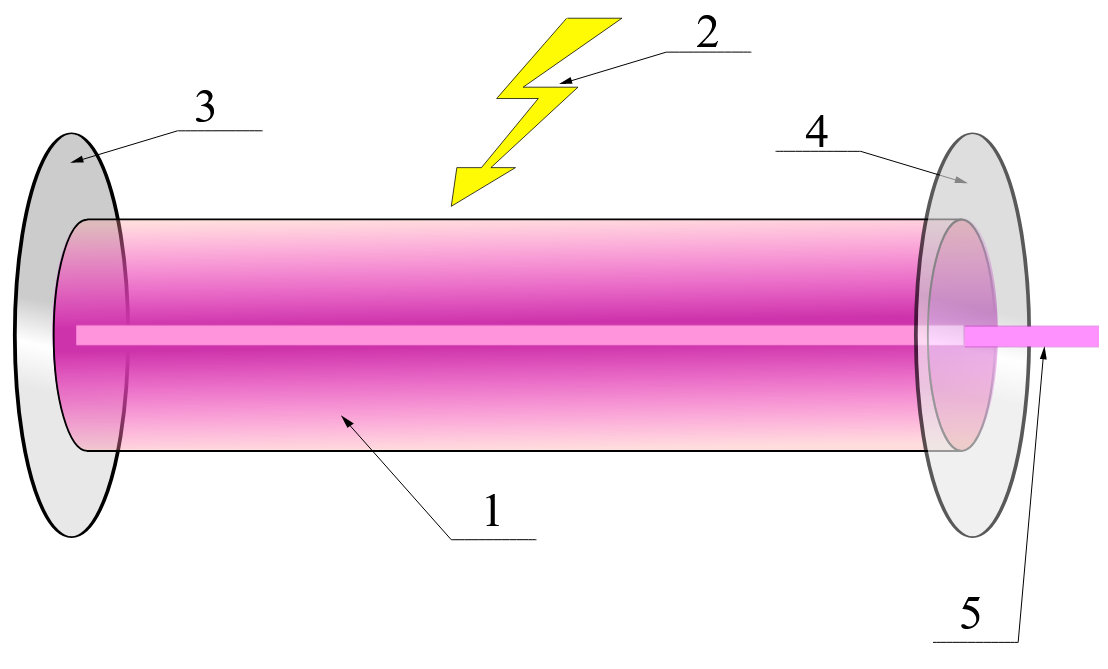
\includegraphics[width=\textwidth]{graphics/Laser_Cavity.png}
%     \caption{Aufnahme der Zählstatistik mit Digitalzähler. \\
%     vertikal = Zerfälle pro Sekunde, horizontal = Messindex}
%     \label{fig:execution:durchfuehrung:zaehlstatistik}
% \end{figure}
\newpage